\section{W\"astlund's construction}\label{sec:wastlund}

\subsection{Brightness and the inverse-square law}

A lamp is a point source emitting a total flux $L$ equally in all directions, and the
observer receives it on a small screen perpendicular to the incoming rays. At distance $r$
the flux is spread over a sphere of area $4\pi r^{2}$, so the brightness per unit area is
\begin{equation}
  B(r)=\frac{L}{4\pi r^{2}}\propto\frac{1}{r^{2}}.
  \label{eq:inverse-square}
\end{equation}
Doubling the distance leaves a quarter of the brightness. Throughout, the distance of a lamp
is measured from the observation point $P$, and a sum of terms $1/d^{2}$ is read as the total
brightness at $P$.

\begin{definition}[lamps, brightness, equivalence]\label{def:lamps}
Fix a point $P$ in the plane, called the \emph{observation point}. A \emph{lamp} is a point
source placed at some $Q\neq P$, and its \emph{brightness at $P$} is the quantity
$1/PQ^{2}$. The \emph{total brightness} of a finite or countable set of lamps is the sum of
their brightnesses. Two lamps $S_{1},S_{2}$ are \emph{equivalent} to a lamp $R$ (at $P$) if
$1/PS_{1}^{2}+1/PS_{2}^{2}=1/PR^{2}$. If a circle through $P$ has centre $O$, the point of the
circle diametrically opposite $P$ is called the \emph{antipodal position} of $P$.
\end{definition}

With this vocabulary, replacing a lamp by two equivalent ones leaves the total brightness
unchanged, and all that must be checked in a replacement step is the inverse Pythagorean
identity of Lemma~\ref{lem:inverse-pythagoras}.

\subsection{The inverse Pythagorean theorem}

\begin{lemma}[inverse Pythagorean]\label{lem:inverse-pythagoras}
Let $a$ and $b$ be the legs of a right triangle, $c$ its hypotenuse, and $h$ the altitude to
the hypotenuse. Then
\begin{equation}
  \frac{1}{h^{2}}
  =\frac{c^{2}}{a^{2}b^{2}}
  =\frac{a^{2}+b^{2}}{a^{2}b^{2}}
  =\frac{1}{a^{2}}+\frac{1}{b^{2}}.
  \label{eq:inverse-pythagoras}
\end{equation}
\end{lemma}

\begin{proof}
Equating the two expressions for the area gives $ab=ch$, hence $c^{2}h^{2}=a^{2}b^{2}$;
substituting $c^{2}=a^{2}+b^{2}$ yields \eqref{eq:inverse-pythagoras}.
\end{proof}

\begin{figure}[htbp]
\centering
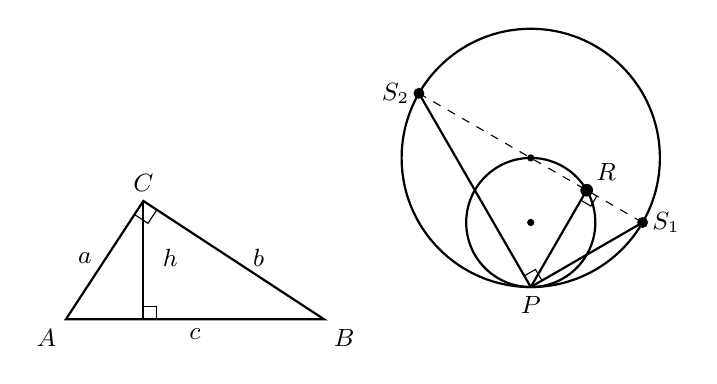
\begin{tikzpicture}[scale=0.82, every node/.style={font=\small}]
  \begin{scope}
    \coordinate (A) at (0,0);
    \coordinate (B) at (4,0);
    \coordinate (C) at (1.2,1.833);
    \coordinate (H) at (1.2,0);
    \draw[thick] (A)--(B)--(C)--cycle;
    \draw[thick] (C)--(H);
    \draw (1.4,0)--(1.4,0.2)--(1.2,0.2);
    \draw (1.063,1.624)--(1.272,1.487)--(1.409,1.696);
    \node[left] at (0.55,0.95) {$a$};
    \node[right] at (2.75,0.95) {$b$};
    \node[right] at (1.35,0.95) {$h$};
    \node[below] at (2,0) {$c$};
    \node[below left] at (A) {$A$};
    \node[below right] at (B) {$B$};
    \node[above] at (C) {$C$};
  \end{scope}

  \begin{scope}[shift={(7.2,0.5)}]
    \coordinate (P) at (0,0);
    \coordinate (O1) at (0,1);
    \coordinate (O2) at (0,2);
    \draw[thick] (O1) circle (1);
    \draw[thick] (O2) circle (2);
    \coordinate (R) at (0.866,1.5);
    \coordinate (S1) at (1.732,1);
    \coordinate (S2) at (-1.732,3);
    \draw[dashed] (S2)--(S1);
    \draw[thick] (P)--(R);
    \draw[thick] (P)--(S1);
    \draw[thick] (P)--(S2);
    \fill (R) circle (2.8pt);
    \fill (S1) circle (2.4pt);
    \fill (S2) circle (2.4pt);
    \fill (O1) circle (1.6pt);
    \fill (O2) circle (1.6pt);
    \draw (0.776,1.344)--(0.932,1.254)--(1.022,1.410);
    \draw (0.173,0.1)--(0.073,0.273)--(-0.1,0.173);
    \node[above right] at (R) {$R$};
    \node[right] at (S1) {$S_1$};
    \node[left] at (S2) {$S_2$};
    \node[below] at (P) {$P$};
  \end{scope}
\end{tikzpicture}
\caption{Left: the inverse Pythagorean theorem. Right: the replacement of
Lemma \ref{lem:replacement}.}
\label{fig:circle-replacement}
\end{figure}

\subsection{One lamp replaced by two equivalent lamps}

\begin{lemma}[replacement]\label{lem:replacement}
Let $C_{1}$ and $C_{2}$ be circles of radii $r_{1}$ and $r_{2}=2r_{1}$, tangent at the
observer $P$, and let $R$ be a lamp on $C_{1}$. The line through $R$ perpendicular to $PR$
meets $C_{2}$ in two points $S_{1}$ and $S_{2}$, and
\begin{equation}
  \underbrace{\frac{1}{PR^{2}}}_{\text{one lamp on }C_{1}}
  \;=\;
  \underbrace{\frac{1}{PS_{1}^{2}}+\frac{1}{PS_{2}^{2}}}_{\text{two lamps on }C_{2}}.
  \label{eq:replacement}
\end{equation}
\end{lemma}

\begin{proof}
The point of $C_{1}$ antipodal to $P$ lies on the line of centres at distance
$2r_{1}=r_{2}$ from $P$, so it is the centre $O_{2}$ of $C_{2}$. Because $PO_{2}$ is a
diameter of $C_{1}$, the angle $PRO_{2}$ is a right angle: the perpendicular to $PR$ at $R$
is the line $RO_{2}$, and it cuts $C_{2}$ in the two endpoints of a diameter. Thus $S_{1}S_{2}$
is a diameter of $C_{2}$, and since $P$ lies on $C_{2}$ the angle $S_{1}PS_{2}$ is a right
angle with $PR$ as the altitude to its hypotenuse. Lemma
\ref{lem:inverse-pythagoras} applied to the triangle $PS_{1}S_{2}$ is exactly
\eqref{eq:replacement}.
\end{proof}

In other words, one lamp on the small circle may be replaced by two lamps on the large one
without changing the brightness at $P$.

\subsection{Doubling: $N$ division points become $2N$}

\begin{lemma}[doubling]\label{lem:doubling}
Place lamps at $N$ equally spaced points of $C_{1}$ and replace each of them by its two
images on $C_{2}$ as in Lemma \ref{lem:replacement}. Those images are the $2N$ equally spaced
points of $C_{2}$ that correspond to them, and the total brightness at $P$ is unchanged.
\end{lemma}

\begin{proof}
The image pair of a lamp $R$ is the diameter of $C_{2}$ through $R$ and $O_{2}$, so the whole
configuration is a set of rays through $O_{2}$. Since $O_{2}$ lies on $C_{1}$, the angles
between consecutive rays are inscribed angles of $C_{1}$ standing on equal chords, hence
equal; the very same angles are central angles of $C_{2}$, so the $2N$ points in which the
rays meet $C_{2}$ cut $C_{2}$ into equal arcs. Brightness is preserved lamp by lamp by
Lemma \ref{lem:replacement}.
\end{proof}

The word \emph{corresponding} matters. The $2N$ points are produced from the $N$ lamps one at
a time; choosing an arbitrary set of $2N$ division points would not preserve the brightness.

\begin{figure}[htbp]
\centering
\begin{tikzpicture}[scale=0.78, every node/.style={font=\small}]
  \coordinate (P) at (0,0);
  \coordinate (O1) at (0,1);
  \coordinate (O2) at (0,2);
  \draw[thick] (O1) circle (1);
  \draw[thick] (O2) circle (2);
  \coordinate (R1) at (0.5,1.866);
  \coordinate (R2) at (0.5,0.134);
  \coordinate (R3) at (-1,1);
  \foreach \a [evaluate=\a as \c using {\a+180}] in {45,105,165}
    \draw[thin] ($(O2)+(\a:2)$)--($(O2)+(\c:2)$);
  \draw[thin] (P)--(R1);
  \draw[thin] (P)--(R2);
  \draw[thin] (P)--(R3);
  \foreach \a in {45,105,165,225,285,345}
    \fill[lampB] ($(O2)+(\a:2)$) circle (2.6pt);
  \fill[lampA] (R1) circle (3.2pt);
  \fill[lampA] (R2) circle (3.2pt);
  \fill[lampA] (R3) circle (3.2pt);
  \fill (O1) circle (1.3pt);
  \fill (O2) circle (1.3pt);
  \node[above left] at ($(O2)+(-0.24,0.24)$) {$O_2$};
  \node[below] at (P) {$P$};
\end{tikzpicture}
\caption{The $3$ division points of the small circle against the corresponding $6$ points of
the large one.}
\label{fig:doubling}
\end{figure}

\subsection{The limit: the circle becomes a line}

Take the circle of circumference $2$, that is, of radius $R_{0}=1/\pi$, with its single lamp
at the point antipodal to $P$. That lamp is at distance $2/\pi$, so the total brightness at
$P$ is
\begin{equation}
  \frac{1}{d^{2}}=\frac{1}{(2/\pi)^{2}}=\frac{\pi^{2}}{4}.
  \label{eq:first-lamp}
\end{equation}

\begin{figure}[H]
\centering
\begin{tikzpicture}[scale=0.78, every node/.style={font=\small}]
  \draw[dashed] (0,0)--(0,4);
  \draw[thick] (0,0.5) circle (0.5);
  \draw[thick] (0,1) circle (1);
  \draw[thick] (0,2) circle (2);
  \draw[thin,dashed] (-1,1)--(1,1);
  \draw[thin,dashed] (1.414,0.586)--(-1.414,3.414);
  \draw[thin,dashed] (-1.414,0.586)--(1.414,3.414);
  \fill[lampB] (1.414,0.586) circle (2.6pt);
  \fill[lampB] (-1.414,0.586) circle (2.6pt);
  \fill[lampB] (1.414,3.414) circle (2.6pt);
  \fill[lampB] (-1.414,3.414) circle (2.6pt);
  \fill[lampB] (1,1) circle (2.8pt);
  \fill[lampB] (-1,1) circle (2.8pt);
  \fill[lampA] (0,1) circle (3.4pt);
  \fill (0,0) circle (1.8pt);
  \node[below left] at (0,0) {$P$};
  \draw[->,thick] (2.5,2)--(3.7,2);
  \node[above,font=\footnotesize] at (3.1,2) {$k\to\infty$};
  \begin{scope}[shift={(7.1,0)}]
    \draw[thick] (-3.4,0)--(3.4,0);
    \fill (0,0) circle (1.8pt);
    \node[above] at (0,0) {$P$};
    \foreach \x/\lab in {-2.8/-7,-2.0/-5,-1.2/-3,-0.4/-1,0.4/1,1.2/3,2.0/5,2.8/7} {
      \fill[lampB] (\x,0) circle (2.6pt);
      \node[below,font=\footnotesize] at (\x,-0.05) {$\lab$};
    }
  \end{scope}
\end{tikzpicture}
\caption{Doubling the radius until the circle flattens into the tangent line.}
\label{fig:doubling-limit}
\end{figure}

Each doubling preserves this total, and after $k$ doublings the lamps of the circle of
circumference $2^{k+1}$ stand at arc-length distances $1,3,5,\dots$ from $P$. As $k\to\infty$
the circle approaches its tangent line at $P$, chord lengths tend to arc lengths, and the
lamps fall at $\pm1,\pm3,\pm5,\dots$ on that line (Figure \ref{fig:doubling-limit}). Hence
\begin{equation}
  2\left(1+\frac{1}{3^{2}}+\frac{1}{5^{2}}+\cdots\right)=\frac{\pi^{2}}{4},
  \label{eq:odd-limit}
\end{equation}
and dividing by $2$ proves Theorem \ref{thm:wastlund}.

\subsection{Back to the Basel problem}

The even terms of \eqref{eq:basel} are $\frac14$ of the whole series, so with
\eqref{eq:odd-sum}
\begin{equation}
  \resizebox{\textwidth}{!}{$
  \begin{array}{r*{21}{c}r}
    &1&&&+&\frac{1}{3^{2}}&&&+&\frac{1}{5^{2}}&&&+&\frac{1}{7^{2}}&&&+&\frac{1}{9^{2}}
    &&&+&\cdots&=\frac{\pi^{2}}{8}\\[14pt]
    S=&1&+&\frac{1}{2^{2}}&+&\frac{1}{3^{2}}&+&\frac{1}{4^{2}}&+&\frac{1}{5^{2}}
    &+&\frac{1}{6^{2}}&+&\frac{1}{7^{2}}&+&\frac{1}{8^{2}}&+&\frac{1}{9^{2}}
    &+&\frac{1}{10^{2}}&+&\cdots&\\[20pt]
    \frac{1}{4}S=&&&\frac{1}{2^{2}}&&&+&\frac{1}{4^{2}}&&&+&\frac{1}{6^{2}}
    &&&+&\frac{1}{8^{2}}&&&+&\frac{1}{10^{2}}&+&\cdots&
  \end{array}$}
  \label{eq:odd-even}
\end{equation}
and therefore $S=\frac{\pi^{2}}{8}\cdot\frac{1}{1-\frac14}=\frac{\pi^{2}}{6}$. This last
computation is the algebraic step that Theorem \ref{thm:direct} below avoids:
\eqref{eq:odd-even} trades $S$ for $\frac34 S$, and with it the information carried by the
figure becomes a subseries.
